\chapter{Evaluation} \label{EvaluationChapter}

In this chapter, we describe our approach to evaluating the new cloud-based execution environment in terms of performance, operating costs, as well as benefits brought to the end user. We describe the results of various benchmarks run against clusters with different configurations and discuss the challenges involved in correctly identifying the most influencing factors for the performance of distributed systems.

Although the specific end goal of the project was providing a new environment for running experiments on AWS from OpenMOLE, we also benchmark the underlying GridScale AWS module separately, since it can be used as a standalone component. We use DoC's\footnote{Imperial College's Department of Computing} HTCondor and Slurm deployments to compare the speed of the new system with a locally hosted cluster.

Throughout the chapter, we delve into considerations about the costs of running specific workflows on AWS and advocate the use of different types of clusters depending on the nature of the workload. To illustrate the benefits of the fully automated job delegation to the cloud, we contrast it with the manual steps previously needed to obtain similar results with other experiment frameworks.

\section{Fully Automated Experiments}

OpenMOLE is now, to our knowledge, the only scientific experimentation framework that allows users to run experiments on commercial cloud environments without any form of configuration beyond providing their credentials. Listing \ref{EnvSwitch} shows how the switch to the cloud is made by injecting the new environment in the workflow instantiation.

\begin{listing}[h]
	\centering
	\begin{minipage}{11.6cm}
		\begin{minted}[frame=single,framesep=2mm,escapeinside=||,baselinestretch=1.15,fontsize=\small,linenos]{scala}
val (t1, t2, t3) = (EmptyTask(), EmptyTask(), EmptyTask())
		
val localhost = LocalEnvironment(threads = 8)
val aws = AWSEnvironment(
  region = "eu-west-1",
  awsUserName = "adrian",
  awsUserId = "434676269080",
  awsKeypairName = "gridscale",
  awsCredentialsPath = "/Users/adrian/.aws/credentials.csv",
  privateKeyPath = "/Users/adrian/.ssh/id_rsa",
  clusterSize = 8
)

val localMole = t1 -- (t2 on localhost) -- t3
val cloudMole = t1 -- (t2 on aws) -- t3
		\end{minted}
	\end{minipage}
	\caption{Creating an experiment ready to run both locally an in the cloud.}
	\label{EnvSwitch}
\end{listing}

As described in the background chapter, other workflow platforms such as Taverna, Galaxy, or the Humman Connectome project have recently started cloud initiatives, but they still rely on a tedious setup on behalf of the user, who is required to follow long and complicated instruction steps \cite{TavernaAWS, GalaxyAWS, Connectome}. 

Although quantifying the ease of use is a subtle task, we have so far been encouraged by feedback. We believe that features such as automatically mapping resources to cloud instances and generating bidding strategies for spot instances bring a quality of life improvement and encourage more users to take advantage of commercial clouds for research.

\section{GridScale Benchmarks}

As the foundation layer OpenMOLE's access to remote resources, GridScale bears significant importance for the overall performance of the application. We believe that benchmarks at this level offer valuable insights into the impact of choosing an appropriate instance type for the master node of the cluster, since the job submission system is evaluated in isolation from other configuration and setup routines employed by higher level systems.

\subsection{Methodology}

In this section, we particularly focus on the rate of at which jobs can be submitted, queried or cancelled on a cluster deployed on Amazon EC2. At this stage, we are not interested in the overall execution time of the submitted jobs, so we do not delegate real work and jobs are just busy-waiting to be cancelled.

Our setup consists of 5 different types of clusters with different types of instances as the single master node. The master is the only job submission controller, so no worker nodes are needed. For each run, we instantiate an \verb|AWSJobService|, submit, query and eventually cancel a number of jobs between 100 and 1000 increasing in steps of 100. 

To ensure a better estimation of the real duration, we repeat each run 10 times and average the results. Table \ref{InstancePrices} shows the specifications and prices of all types of instances used in this chapter.

\begin{table}[h]
\centering
\begin{adjustbox}{width=1\textwidth}
\begin{tabular}{ccccccc}
 &  &  &  &  & \multicolumn{2}{c}{\textbf{Price (\$ per hour)}} \\ \cline{6-7} 
\textbf{Instance Type} & \textbf{Memory (GB)} & \textbf{ECUs\footnote{An EC2 Compute Unit is the approximate equivalent of a 1.0-1.2 GHz 2007 Intel Xeon}} & \textbf{vCPUs\footnote{Virtual CPUs}} & \multicolumn{1}{c|}{\textbf{Network Performance}} & \multicolumn{1}{c|}{\textbf{Spot}} & \multicolumn{1}{c|}{\textbf{On-Demand}} \\ \hline
\multicolumn{1}{|c|}{m1.small} & \multicolumn{1}{c|}{1.7} & \multicolumn{1}{c|}{1} & \multicolumn{1}{c|}{1} & \multicolumn{1}{c|}{Low (125 Mbps)} & \multicolumn{1}{c|}{0.01} & \multicolumn{1}{c|}{0.047} \\ \hline
\multicolumn{1}{|c|}{m1.medium} & \multicolumn{1}{c|}{3.75} & \multicolumn{1}{c|}{2} & \multicolumn{1}{c|}{1} & \multicolumn{1}{c|}{Moderate (250 Mbps)} & \multicolumn{1}{c|}{0.01} & \multicolumn{1}{c|}{0.095} \\ \hline
\multicolumn{1}{|c|}{m3.medium} & \multicolumn{1}{c|}{3.75} & \multicolumn{1}{c|}{3} & \multicolumn{1}{c|}{1} & \multicolumn{1}{c|}{Moderate (300 Mbps)} & \multicolumn{1}{c|}{0.01} & \multicolumn{1}{c|}{0.073} \\ \hline
\multicolumn{1}{|c|}{c1.medium} & \multicolumn{1}{c|}{1.7} & \multicolumn{1}{c|}{5} & \multicolumn{1}{c|}{2} & \multicolumn{1}{c|}{Moderate (250 Mbps)} & \multicolumn{1}{c|}{0.02} & \multicolumn{1}{c|}{0.148} \\ \hline
\multicolumn{1}{|c|}{m1.xlarge} & \multicolumn{1}{c|}{15} & \multicolumn{1}{c|}{8} & \multicolumn{1}{c|}{4} & \multicolumn{1}{c|}{High (1000 Mbps)} & \multicolumn{1}{c|}{0.04} & \multicolumn{1}{c|}{0.379} \\ \hline
\multicolumn{1}{|c|}{c3.xlarge} & \multicolumn{1}{c|}{7.5} & \multicolumn{1}{c|}{14} & \multicolumn{1}{c|}{4} & \multicolumn{1}{c|}{Moderate (500 Mbps)} & \multicolumn{1}{c|}{0.043} & \multicolumn{1}{c|}{0.239} \\ \hline
\multicolumn{1}{|c|}{c3.4xlarge} & \multicolumn{1}{c|}{30} & \multicolumn{1}{c|}{62} & \multicolumn{1}{c|}{16} & \multicolumn{1}{c|}{High (2 Gbps)} & \multicolumn{1}{c|}{0.168} & \multicolumn{1}{c|}{0.953} \\ \hline
\multicolumn{1}{|c|}{c3.8xlarge} & \multicolumn{1}{c|}{60} & \multicolumn{1}{c|}{132} & \multicolumn{1}{c|}{36} & \multicolumn{1}{c|}{Very High (10 Gbps)} & \multicolumn{1}{c|}{0.327} & \multicolumn{1}{c|}{1.906} \\ \hline
\end{tabular}
\end{adjustbox}
\caption{Performances and prices of AWS EC2 instances. Prices as of June 2016 in EU West \cite{EC2}.}
\label{InstancePrices}
\end{table}

At the moment, not all GridScale modules support batching commands sent to the submission controller via multiple sessions within the same SSH connection, so we consider two main scenarios based on whether operations to the master are transmitted using only one or more sessions per TCP connection.

\subsection{Results}

In the case of a single session per connection, we also compare the 5 master nodes of the GridScale SGE cluster with the manager of the HTCondor in DoC. This is an Intel Xeon E5-2470 with 32GB RAM and 16 virtual cores running at 2.3GHz. 

\begin{figure}[H]
	\centering
	\minipage{0.49\textwidth}
		\subfloat[][]{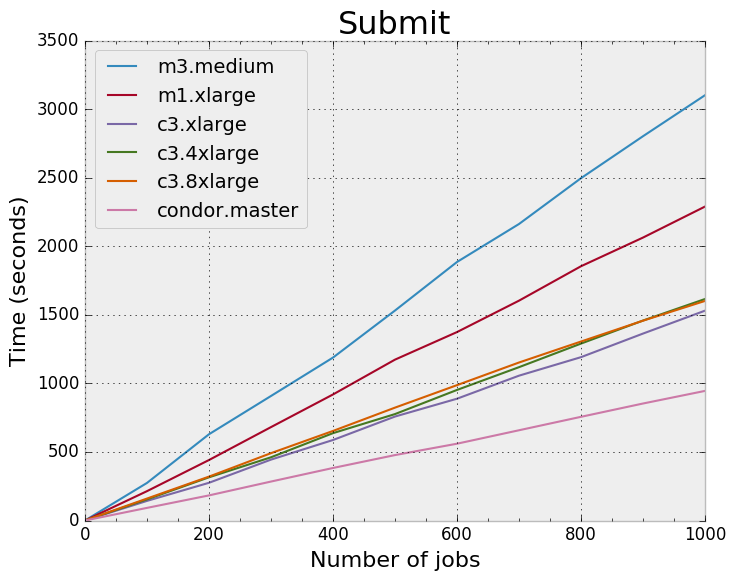
\includegraphics[width=1\linewidth]{GridScaleSubmit.png}}
	\endminipage \vfill
	\minipage{0.49\textwidth}
		\subfloat[][]{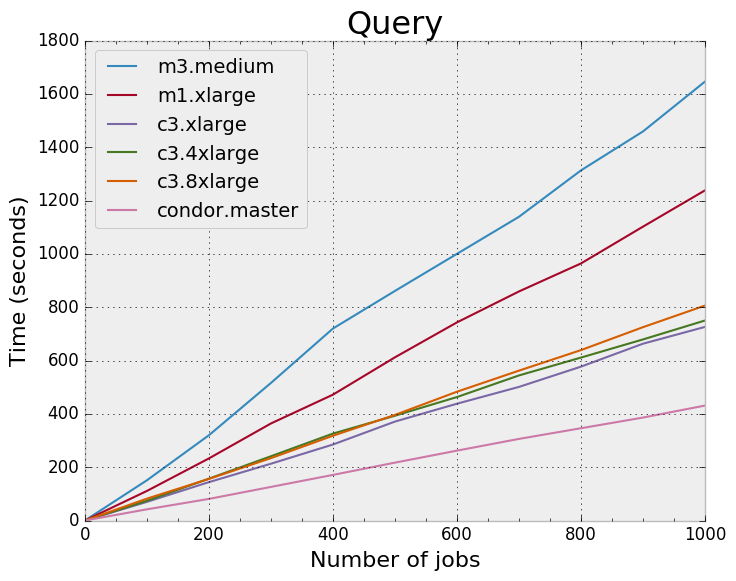
\includegraphics[width=1\linewidth]{GridScaleQuery.png}}
	\endminipage \hfill
	\minipage{0.49\textwidth}
		\subfloat[][]{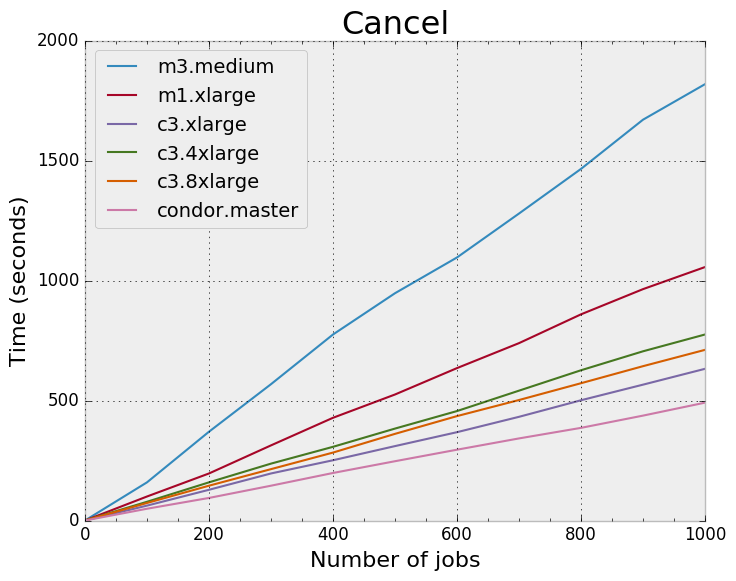
\includegraphics[width=1\linewidth]{GridScaleCancel.png}}
	\endminipage \hfill
	\caption{Comparison for submission, query and cancellation times for an increasing number of jobs on different types of master nodes.}
	\label{SingleSession}
\end{figure}

Figure \ref{SingleSession} shows that submissions to the HTCondor server are significantly faster for all instructions, partly due to the high bandwidth on the local network, but mostly thanks to the very low latency, which reduces the time needed to establish an SSH connection. While the \verb|m3.medium| clearly lags behind given its low bandwidth, the three high-CPU \verb|c3| instances exhibit close performance and are faster than the high-throughput \verb|m1.xlarge| instance, indicating that bandwidth only has diminishing returns and the CPU is more important, while latency remains a constant factor.

\todo[]{Async}

\section{OpenMOLE Workflow Benchmarks}



\section{Spot Clusters}

\section{Challenges and Limitations}

\todo[inline]{Amazon cagey with number of spots - can contact them to increase it - The total number of Spot instance requests 20 per region}

\todo[inline]{Results influenced by the fact that we couldn't really use the best available machines due to budget. Usually, benchmarks are run on really powerful machines.}

\todo[inline]{Make the point that it is expected for experiments to be slower on the cloud, since academic grids and local clusters usually benefit from way above average machines or even supercomputers, which are clearly unaffordable in a commercial setting. So being in the same order of magnitude is alright}

\todo[inline]{Not worth ever using reserved machines - 12\% cheaper if reserved 3 years in advance}

\todo[inline]{Show performances of all instances used to experiment with}

\section{Fluff}

As described in the project plan, we plan to develop the project incrementally, by having an early functional implementation that we can afterwards iteratively improve. Since we assume a stable, albeit limited, product at each iteration, we will also be able to perform evaluation at each stage. The results of the benchmarks should guide the further development of the project by helping us to identify non-optimal solutions, bugs, or negative user feedback.

The main performance benchmark that we plan to run is against the current speed and resource utilisation of OpenMOLE when submitting jobs to grids and clusters. This will allow us to find the performance problems generated exclusively by the deployment of jobs to the cloud and point to potential bottlenecks. However, we expect performance to slightly decrease, given that standard machines available in cloud environments are less powerful than those designed specifically for high performance computing purposes and used in common scientific grids and clusters \cite{Juve2009}.

We consider direct comparison with other workflow systems not to be a very reliable performance indicator for the new cloud integration, since results would be influenced by the overall structure of the system. We also rate it as a stretch goal because studying the workflow definition procedures for each different workflow systems can be time consuming and most non-generic platforms refer to contextual information in fields that we are not familiar with.

Quantifying the ease of use and quality of the implementation is a more subtle task. Since one of the goals of the project is to achieve automation of deploying clusters and running jobs in the cloud, we can measure the positive impact on the user experience by the degree to which full automation is achieved. Requiring too much user configuration is one of the main drawbacks of competing workflow management and we believe that overcoming this can objectively be considered a success.

OpenMOLE and GridScale are open-source projects, so the implementation quality factor can potentially be evaluated by the level of interference with other components of the modular architecture. Although fragile design and implementation bugs should be observed in the early development stage, we plan to measure the reliability of the new workflow execution environment by running several stress tests against the current execution environments.